\documentclass{article}
\usepackage{amsmath}
\usepackage{amsfonts}
\usepackage{amssymb}
\usepackage{enumitem}
\usepackage{tikz}
\usepackage{mathtools}

\usetikzlibrary{arrows}

\title{MATH 222 - Assignment 4}
\date{March 2017}
\author{Daniel Frankcom}

\begin{document}
	\pagenumbering{gobble}
	\maketitle
	\setlength{\parindent}{0pt}
	\newcommand{\forceindent}{\leavevmode{\parindent=72pt\indent}}
	\newpage
	\pagenumbering{arabic}
	
	\begin{enumerate}
		
		\item 
		\begin{enumerate}
			\item In order for a relation to be both symmetric and antisymmetric, it must only contain reflexive elements. For each reflexive pair $(x,x)$, there are 2 options: either the pair is in the relation, or it is not.
			\newline $\therefore$ there are $2^n$ relations on $A$ that fulfill the requirements
			\item If $R$ is a relation on $A$ that is antisymmetric, then it may not contain any 2 pairs such that $(x,y)$ and $(y,x)$ are both in $R$ unless $x=y$.
			\newline $\therefore$ we can count the number of elements in the upper diagonal half of the corresponding relation matrix.
			\newline This is equivalent to $\sum\limits_{i=1}^{n}i=\frac{n(n+1)}{2}$
			\item For each pair, either $(x,y)$ or $(y,x)$ may be in $R$, unless $x=y$.
			\newline $\therefore$ there are $\frac{n(n+1)}{2}-n=\frac{n(n-1)}{2}$ pairs that may be swapped out for their inverse.
			\newline As in part (a), we have 2 options for each of our pairs, so we have $2^\frac{n(n-1)}{2}$ relations
			\item If $R$ has domain $A$ and is a function, then each element may map to only 1 other element in $A$, by the definition of a function. 
			\newline Since $R$ is reflexive, for every $x\in A$ the pair $(x,x)$ must be in $R$.
			\newline Since every value in the domain is already mapped to itself, we know that no value can map to another due to our function restriction.
			\newline $\therefore R$ is made up of all of the reflexive pairs $(x,x)$ where $x\in A$
		\end{enumerate}
	
		\item 
		\begin{enumerate}
			\item \mbox{}
			\newline
			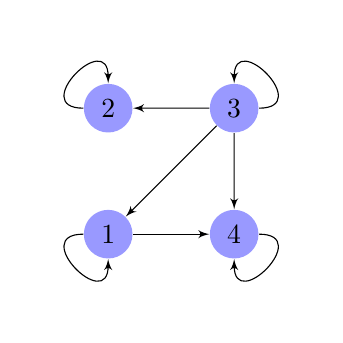
\begin{tikzpicture}
			[scale=.8,auto=left,every node/.style={circle,fill=blue!40}, edge/.style={->,> = latex'}]
			\node (n1) at (0,0)  {1};
			\node (n2) at (0,2)  {2};
			\node (n3) at (2,2)  {3};
			\node (n4) at (2,0)  {4};
			
			\foreach \from/\to in {n1/n4,n3/n4,n3/n1,n3/n2}
			\draw[edge] (\from) to (\to);
			
			\draw[edge] (n1) to [out=180,in=270,looseness=4] (n1);
			\draw[edge] (n2) to [out=180,in=90,looseness=4] (n2);
			\draw[edge] (n3) to [out=360,in=90,looseness=4] (n3);
			\draw[edge] (n4) to [out=360,in=270,looseness=4] (n4);
			\end{tikzpicture}
			
			\item \mbox{}
			\newline
			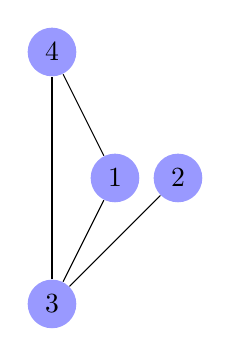
\begin{tikzpicture}
			[scale=.8,auto=left,every node/.style={circle,fill=blue!40}, edge/.style={-,> = latex'}]
			\node (n1) at (1,2)  {1};
			\node (n2) at (2,2)  {2};
			\node (n3) at (0,0)  {3};
			\node (n4) at (0,4)  {4};
			
			\foreach \from/\to in {n1/n4,n3/n4,n3/n1,n3/n2}
			\draw[edge] (\from) to (\to);

			\end{tikzpicture}
			
			\newpage
			\item A total order must be antisymmetric, but must also contain at least one pair for every $x,y\in A$. There are currently 2 sets of pairs that are not included in $R$, these being $(2,1)/(1,2)$ and $(2,4)/(4,2)$.
			\newline For each of these 2 pairs there are 2 choices, with that choice being which will be in our total order.
			\newline $\therefore$ there are $2^2=4$ total orders containing our partial order
		\end{enumerate}
	
		\item
		\begin{enumerate}
			\item In order for $R$ to be an equivalence relation, it must be symmetric, reflexive, and transitive.
			\begin{enumerate}
				\item Multiplication is commutative, so if $xy>0$, we know that $yx>0$
				\newline This means that if $xRy$ then $yRx$
				\newline $\therefore R$ is symmetric
				
				\item Given any non-zero numbers $x,y$ we know that $xy\neq0$
				\newline $\therefore$ the product must be less than 0 or greater than 0
				\newline For any $x$ we know $xRx$ since $x^2$ will also be positive
				\newline $\therefore$ $R$ is reflexive
				
				\item If $xRy$ then $x$ and $y$ are both positive or both negative
				\newline If $yRz$ also, then $z$ has the same sign as both $x$ and $y$
				\newline If this is the case, then $xRz$ since they have the same sign
				\newline $\therefore R$ is transitive
			\end{enumerate}
			$\therefore R$ is an equivalence relation on $S$
			\newline [1] and [-1] are examples of equivalence classes on $R$ than give a partition of $S$, as the 2 partitions in this case are the set of positive numbers and the set of negative numbers.
			
			\item $R_2$ is not an equivalence relation because $x^2$ is always positive, and therefore not in $R_2$. This means that the relation is not reflexive, and is therefore not an equivalence relation.
		\end{enumerate}
		
		\item
		\begin{enumerate}
			\item In order for $R_Y$ to be a partial order on $Y$ it must be anti-symmetric, reflexive, and transitive.
			\begin{enumerate}
				\item Since for any $a,b\in Y$, $(a,b)$ is in $R_Y$ if and only if it is in $R$, then $(b,a)$ cannot also be in $R_Y$ since $R$ is already a partial order, and therefore cannot contain $(b,a)$
				\newline $\therefore R_Y$ is anti-symmetric
				
				\item Since for any $a\in Y$, $(a,a)$ is in $R$, we know that it is also in $R_Y$ since both of the inclusion conditions are met.
				\newline $\therefore R_Y$ is reflexive
				
				\item Since for any $a,b,c\in Y$, if $(a,b)$ and $(b,c)$ are both in $R$ then we know that $(a,c)$ must also be in $R$ since it is a partial order
				\newline $\therefore R_Y$ is transitive
			\end{enumerate}
			$\therefore$ $R_Y$ is a partial order on $Y$
			
			\newpage
			\item For $R$ to be a total order, then for any $x,y\in X$ either the pair $(x,y)$ or $(y,x)$ is in $R$
			\newline If this is the case, then for any $x,y\in Y$ either $(x,y)$ or $(y,x)$ will be in $R_Y$
			\newline $\therefore R_Y$ is a total order on $Y$
		\end{enumerate}
	
		\item
		\begin{enumerate}
			\item $g(x)=\frac{x^3}{1-x^2}$
			\newline $=x^3\frac{1}{1-x^2}$
			\newline $=x^3\sum\limits_{n=0}^{\infty}(x^2)^n$
			\newline $=x^3\sum\limits_{n=0}^{\infty}x^{2n}$
			\newline $=x^3(1+x^2+x^4+...)$
			\newline $=x^3+x^5+x^7+...$
			\newline $0,0,0,1,0,1,0,...$
			
			\item $g(x)=(4x-1)^3$
			\newline $=-(1-4x)^3$
			\newline $=-\sum\limits_{n=0}^{3}{{3}\choose{n}}(-4x)^n$
			\newline $=-[1+3(-4x)+3(-4x)^2+(-4x)^3]$
			\newline $=-(1-12x+48x^2-64x^3)$
			\newline $=-1+12x-48x^2+64x^3$
			\newline $-1,12,-48,64,0,0,...$
			
			\item $g(x)=\frac{1-x}{1+x}$
			\newline $=\frac{1}{1+x}-x\frac{1}{1+x}$
			\newline $=\sum\limits_{n=0}^{\infty}(-1)^nx^n-x\sum\limits_{n=0}^{\infty}(-1)^nx^n$
			\newline $=(1-x+x^2-x^3+...)-x(1-x+x^2-x^3+...)$
			\newline $=(1-x+x^2-x^3+...)-(x-x^2+x^3-x^4+...)$
			\newline $=1-2x+2x^2-2x^3+...$
			\newline $1,-2,2,-2,2,...$
		\end{enumerate}
	
		\item
		\begin{enumerate}
			\item This sequence looks similar to $g(x)=\frac{1}{1+x}$ in that the signs alternate
			\newline This gives us $1,-1,1,-1,...$
			\newline Unfortunately the corresponding sequence does not start with 0, but we can fix this by amending our guess to $g(x)=\frac{x}{1+x}$
			\newline This gives us $0,1,-1,1,-1,...$
			\newline Now we need to deal with the increasing powers of 2. Since these numbers are clearly tied to n, we can multiply x in the denominator by 2, so that when the sum $\sum\limits_{n=0}^{\infty}(-1)^nx^n$ is evaluated we will get $(2x)^n$ and subsequently $2^n$ in front of our $x$
			\newline $\therefore g(x)=\frac{x}{1+2x}$ 
			
			\newpage
			\item It is immediately apparent that some values of n are skipped in this sequence, but we will start with $g(x)=\frac{1}{1+x}$ once again due to the alternating signs
			\newline This gives us $1,-1,1,-1,...$
			\newline We will perform the same procedure as above by making $g(x)=\frac{x}{1+x}$
			\newline This give us $0,1,-1,1,-1,...$
			\newline Now we must deal with the fact that numbers are skipped. Since every other number is skipped, we are dealing with $x^{2n}$ in our sum. To accomplish this in our generating function, we can square $x$ in the denominator
			\newline $\therefore g(x)=\frac{x}{1+x^2}$
		\end{enumerate}
		
	\end{enumerate}
\end{document}